%%%%%%%%%%%%%%%%%%%%%%%%%%%%%%%%%%%%%%%%% 
% Beamer Presentation
% LaTeX Template
% Version 1.0 (10/11/12)
% 
% This template has been downloaded from:
% http://www.LaTeXTemplates.com
% 
% License:
% CC BY-NC-SA 3.0 (http://creativecommons.org/licenses/by-nc-sa/3.0/)
% 
%%%%%%%%%%%%%%%%%%%%%%%%%%%%%%%%%%%%%%%%% 

% ----------------------------------------------------------------------------------------
%	PACKAGES AND THEMES
% ----------------------------------------------------------------------------------------

\documentclass{beamer}

\mode<presentation> {

  % The Beamer class comes with a number of default slide themes
  % which change the colors and layouts of slides. Below this is a list
  % of all the themes, uncomment each in turn to see what they look like.

  % \usetheme{default}
  % \usetheme{AnnArbor}
  % \usetheme{Antibes}
  % \usetheme{Bergen}
  \usetheme{Berkeley}
  % \usetheme{Berlin}
  % \usetheme{Boadilla}
  % \usetheme{CambridgeUS}
  % \usetheme{Copenhagen}
  % \usetheme{Darmstadt}
  % \usetheme{Dresden}
  % \usetheme{Frankfurt}
  % \usetheme{Goettingen}
  % \usetheme{Hannover}
  % \usetheme{Ilmenau}
  % \usetheme{JuanLesPins}
  % \usetheme{Luebeck}
  % \usetheme{Madrid}
  % \usetheme{Malmoe}
  % \usetheme{Marburg}
  % \usetheme{Montpellier}
  % \usetheme{PaloAlto}
  % \usetheme{Pittsburgh}
  % \usetheme{Rochester}
  % \usetheme{Singapore}
  % \usetheme{Szeged}
  % \usetheme{Warsaw}

  % As well as themes, the Beamer class has a number of color themes
  % for any slide theme. Uncomment each of these in turn to see how it
  % changes the colors of your current slide theme.

  % \usecolortheme{albatross}
  % \usecolortheme{beaver}
  % \usecolortheme{beetle}
  % \usecolortheme{crane}
  % \usecolortheme{dolphin}
  % \usecolortheme{dove}
  % \usecolortheme{fly}
  % \usecolortheme{lily}
  % \usecolortheme{orchid}
  % \usecolortheme{rose}
  % \usecolortheme{seagull}
  % \usecolortheme{seahorse}
  % \usecolortheme{whale}
  % \usecolortheme{wolverine}

  % \setbeamertemplate{footline} % To remove the footer line in all slides uncomment this line
  % \setbeamertemplate{footline}[page number] % To replace the footer line in all slides with a simple slide count uncomment this line

  % \setbeamertemplate{navigation symbols}{} % To remove the navigation symbols from the bottom of all slides uncomment this line
}

\usepackage{graphicx} % Allows including images
\usepackage{booktabs} % Allows the use of \toprule, \midrule and \bottomrule in tables

% ---------------------------------------------------------------
%	TITLE PAGE
% ---------------------------------------------------------------

\title[GLSL Part 1]{Intro to GLSL and Shaders} % The short title appears at the bottom of every slide, the full title is only on the title page

\author{Dane Christensen, Brigham H. Keys, Esq.} % Your name
\institute[BYU-Idaho] % Your institution as it will appear on the bottom of every slide, may be shorthand to save space
{
  Brigham Young University - Idaho\\
  \medskip
  \textit{bkeys@bkeys.org} % Your email address
}
\date{\today} % Date, can be changed to a custom date

\begin{document}

% -------------BEGIN SLIDE------------------------
\begin{frame}

  \titlepage % Print the title page as the first slide
  
\includegraphics[scale=.1]{../logo.png}
\end{frame}
% -------------END SLIDE--------------------------


% ------------------------------------------------------------------------
%	PRESENTATION SLIDES
% ------------------------------------------------------------------------

% ------------------------------------------------
\section{About Shaders}
% ------------------------------------------------

% -------------BEGIN SLIDE------------------------
\begin{frame}

  \frametitle{What are shaders?}

  \begin{itemize}
  \item There are multiple shading langauges, such as HLSL, GLSL, and Kronos is releasing SPIR-V later this year.
  \item Just like anything you write in C++, shaders have source code, files, and are compiled.
  \item GLSL's syntax is very similar to the C programming language, so hopefully the learning curve will be minimal.
  \item Shaders are stored in IDs, which are ints.
  \item In this slide show we present how to compile a shader in it's own seperate source file, as it's own seperate program.
  \item Shaders reside entirely in the GPU when they are ran
  \end{itemize}

\end{frame}
% -------------END SLIDE--------------------------

% -------------BEGIN SLIDE------------------------
\begin{frame}

  \frametitle{Types of Shaders}
  There are two different kinds of shaders that together create a shader program, both are required for the shader to work.\\
  Chances are you are not going to need to write your own shader, as there are plenty of well written shaders online.\\
  \begin{block}{Vertex Shaders}
    States the position of a vertex (Very similar to a GL translation). Earlier when we used glVertex3f, that was a vertex shader. It tells OpenGL which points in 3D space we want to shade inbetween.
  \end{block}

  \begin{block}{Fragment Shaders}
    Tells OpenGL, how we want to shade pixels on our screen. OpenGL is a very low level API so we can shade on a per-pixel basis if we wish.
  \end{block}
\end{frame}
% -------------END SLIDE--------------------------

% -------------BEGIN SLIDE------------------------
\begin{frame}

  \frametitle{About making a shader program}

  \begin{itemize}
  \item Compiling a shader successfully gets us an ID for that shader.
  \item Requiring both a fragment shader, and a vertex shader.
  \item Compiler errors are possible, but checking for then is optional.
  \item A shader program is created by linking the fragment shader to the vertex shader.
  \item The shader program itself has an ID.
  \item Very rarely can a shader not be re-used
  \end{itemize}

\end{frame}
% -------------END SLIDE--------------------------


% ------------------------------------------------
\section{Utilizing Shaders}
% ------------------------------------------------

% -------------BEGIN SLIDE------------------------
\begin{frame}

  \frametitle{Examples of GLSL Program}
  \begin{block}{Vertex Shader}
    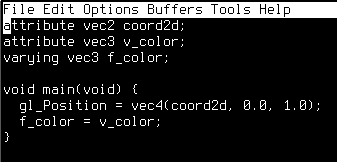
\includegraphics[scale=.4]{vert_shader.png}
  \end{block}
  \begin{block}{Fragment Shader}
    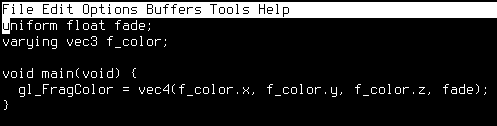
\includegraphics[scale=.4]{frag_shader.png}
  \end{block}
\end{frame}
% -------------END SLIDE--------------------------

% -------------BEGIN SLIDE------------------------
\begin{frame}

  \frametitle{Compute Shaders}
Most modern GPUs have many tiny cores optimized for smaller calculations. Since shaders reside entirely on the GPU, we can run a shader that performs only mathmatical calculations, \emph{using the GPU for tasks that are not graphical at all}. APIs like Nvidia's CUDA give the developer an interface to do this in.
\begin{block}{What is a compute shader?}
  \begin{itemize}
\item Do not have to shade anything on the screen at all.
\item The shader mostly performs various mathmatical calculations.
\item It enables the developer to put the load on the GPU for performing tasks better optimized for a GPU, or anything they want to put in the shader
  \end{itemize}
\end{block}
\end{frame}
% -------------END SLIDE--------------------------

% -------------BEGIN SLIDE------------------------
\begin{frame}

  \frametitle{Compiling into a shader}

  \begin{block}{Getting the program ID}
    The function needed to compile and get the ID for the shader is\\
    GLuint glCreateShader(GL\_VERTEX\_SHADER);
  \end{block}

  \begin{block}{Create the shader program}
    The function to bind the source code to the shader (this must happen before compilation)\\
    void glShaderSource(GLuint shader,
    GLsizei count,
    const GLchar **string,
    const GLint *length);
  \end{block}

  \begin{block}{Create our shader!}
    Now we compile ths shader with:\\
    glCompileShader(GLuint\_ID);
  \end{block}

\end{frame}
% -------------END SLIDE--------------------------

% -------------BEGIN SLIDE------------------------
\begin{frame}

  \frametitle{Using our shader we created}

  \begin{block}{Let OpenGL know you are using a shader}
    void GLuint glCreateProgram();\\
    This behaves very much like a constructor.
  \end{block}

  \begin{block}{We now attach both shaders to the program}
    void glAttachShader(program\_ID, shader\_ID);
  \end{block}

  \begin{block}{Create our shader program, put it together}
    void glLinkProgram(program\_ID);
  \end{block}

  \begin{block}{Place this before you begin to render}
    void glUseProgram(program\_ID);
  \end{block}

\end{frame}
% -------------END SLIDE--------------------------

% -------------BEGIN SLIDE------------------------
\begin{frame}
  \frametitle{References}

A complete class for shader programs can be found in the following link under the files shader.cpp and shader.h\\
\url{https://github.com/BennyQBD/ModernOpenGLTutorial}\\

  \footnotesize{
    \begin{thebibliography}{99}

    \bibitem[OpenGL, 2015]{p1} https://www.opengl.org/ (2015)
    \end{thebibliography}
  }
  
\includegraphics[scale=.33]{../cc.png}

\end{frame}
% -------------END SLIDE--------------------------
\end{document} 
